% THIS IS SIGPROC-SP.TEX - VERSION 3.1
% WORKS WITH V3.2SP OF ACM_PROC_ARTICLE-SP.CLS
% APRIL 2009
%
% It is an example file showing how to use the 'acm_proc_article-sp.cls' V3.2SP
% LaTeX2e document class file for Conference Proceedings submissions.
% ----------------------------------------------------------------------------------------------------------------
% This .tex file (and associated .cls V3.2SP) *DOES NOT* produce:
%       1) The Permission Statement
%       2) The Conference (location) Info information
%       3) The Copyright Line with ACM data
%       4) Page numbering
% ---------------------------------------------------------------------------------------------------------------
% It is an example which *does* use the .bib file (from which the .bbl file
% is produced).
% REMEMBER HOWEVER: After having produced the .bbl file,
% and prior to final submission,
% you need to 'insert'  your .bbl file into your source .tex file so as to provide
% ONE 'self-contained' source file.
%
% Questions regarding SIGS should be sent to
% Adrienne Griscti ---> griscti@acm.org
%
% Questions/suggestions regarding the guidelines, .tex and .cls files, etc. to
% Gerald Murray ---> murray@hq.acm.org
%
% For tracking purposes - this is V3.1SP - APRIL 2009

\newcommand{\squishlist}{
  \begin{list}{$\bullet$}{
      \setlength{\itemsep}{2pt}       \setlength{\parsep}{3pt}
      \setlength{\topsep}{3pt}        \setlength{\partopsep}{0pt}
      \setlength{\leftmargin}{3.5mm}  \setlength{\labelwidth}{1em}
      \setlength{\labelsep}{0.5em} } }

\newcommand{\squishend}{\end{list}}

\documentclass{acm_proc_article-sp}

\begin{document}

\title{SolocoRank: Using Social Signals for Local Place Quality}
%\subtitle{[Extended Abstract]
%\titlenote{A full version of this paper is available as
%\textit{Author's Guide to Preparing ACM SIG Proceedings Using
%\LaTeX$2_\epsilon$\ and BibTeX} at
%\texttt{www.acm.org/eaddress.htm}}}
%
% You need the command \numberofauthors to handle the 'placement
% and alignment' of the authors beneath the title.
%
% For aesthetic reasons, we recommend 'three authors at a time'
% i.e. three 'name/affiliation blocks' be placed beneath the title.
%
% NOTE: You are NOT restricted in how many 'rows' of
% "name/affiliations" may appear. We just ask that you restrict
% the number of 'columns' to three.
%
% Because of the available 'opening page real-estate'
% we ask you to refrain from putting more than six authors
% (two rows with three columns) beneath the article title.
% More than six makes the first-page appear very cluttered indeed.
%
% Use the \alignauthor commands to handle the names
% and affiliations for an 'aesthetic maximum' of six authors.
% Add names, affiliations, addresses for
% the seventh etc. author(s) as the argument for the
% \additionalauthors command.
% These 'additional authors' will be output/set for you
% without further effort on your part as the last section in
% the body of your article BEFORE References or any Appendices.

%\numberofauthors{4} %  in this sample file, there are a *total*
% of EIGHT authors. SIX appear on the 'first-page' (for formatting
% reasons) and the remaining two appear in the \additionalauthors section.
%
% You can go ahead and credit any number of authors here,
% e.g. one 'row of three' or two rows (consisting of one row of three
% and a second row of one, two or three).
%
% The command \alignauthor (no curly braces needed) should
% precede each author name, affiliation/snail-mail address and
% e-mail address. Additionally, tag each line of
% affiliation/address with \affaddr, and tag the
% e-mail address with \email.
%
\numberofauthors{4}
\author{
% 1st. author
\alignauthor Raymond Cheng\\
       \affaddr{University of Washington}\\
       \email{ryscheng@cs.washington.edu}
\and % use '\and' if you need 'another row' of author names
% 2nd. author
\alignauthor Michael Schueppert \\
       \affaddr{Google Inc.}\\
       \email{mschueppert@google.com}
% 3rd. author
\alignauthor Hila Becker \\
       \affaddr{Google Inc.}\\
       \email{hila@google.com}
% 4th. author
\alignauthor Mayur Thakur \\
       \affaddr{Google Inc.}\\
       \email{mayurthakur@google.com}
}
% There's nothing stopping you putting the seventh, eighth, etc.
% author on the opening page (as the 'third row') but we ask,
% for aesthetic reasons that you place these 'additional authors'
% in the \additional authors block, viz.
%\additionalauthors{Additional authors: John Smith (The Th{\o}rv{\"a}ld Group,
%email: {\texttt{jsmith@affiliation.org}}) and Julius P.~Kumquat
%(The Kumquat Consortium, email: {\texttt{jpkumquat@consortium.net}}).}
%\date{30 July 1999}
% Just remember to make sure that the TOTAL number of authors
% is the number that will appear on the first page PLUS the
% number that will appear in the \additionalauthors section.

\maketitle
\begin{abstract}
User-contributed Web data contains rich information about
the physical establishments in the real-world, such as restaurants and hotels.
Our goal is to leverage this growing source of data on the Web
in order to improve the quality of restaurant recommendations from local search engines.
We do so by generating a query-independent score of quality for all establishments in the US.
Search engines that rely purely on raw user-generated reviews suffer from three major limitations.
First, the same top places are reinforced at the head of results, causing bias towards places
that were introduced first. 
Second, user-generated review scores offer very little insight into the establishment's quality.
Scores are limited to fairly coarse resolution, such as discrete values from 0 to 5,
and research has shown that scores tend to be biased towards high scores.
Lastly, user-generated reviews are notoriously noisy, as each person may hold very different
standards in what the value of each star means.
User-generated reviews alone act as a weak signal for indicating the quality of an establishment,
and search engines that use them naively can lead to poor results.
Instead, we demonstrate that many of these problems can be mitigated
by leveraging editorial review services, such as Zagat.

We built a new learn-to-rank system, named \emph{SolocoRank}, trained on
scores from editorial review services to more accurately rank all establishments.
\emph{SolocoRank} leverages a variety of signals on the Web, including 
new social media data sources such as check-ins and microblogs.
Our approach has shown to accurately predict editorial review scores.
When trained on Zagat scores, we show that \emph{SolocoRank} exhibits significant performance
gains in ranking establishments, even for the long-tail
of lower quality establishments.

\end{abstract}

% A category with the (minimum) three required fields
\category{H.3.3}{Information Search and Retrieval}{Retrieval Models}
%A category including the fourth, optional field follows...
%\category{D.2.8}{Software Engineering}{Metrics}[complexity measures, performance measures]
\terms{Algorithms, Measurement, Performance, Experimentation}
\keywords{social media, place quality, local ranking} % NOT required for Proceedings

\vspace{0.1in}
\section{Introduction}
\label{sec:introduction}

Ranking physical establishments, such as restaurants and bars, is a problem
of significant commerical importance.
An understanding of an establishment's quality has wide applicability in improving
local search, recommendation systems, and mapping software.
However, broadly quantifying establishment quality at scale is a particularly difficult
research problem at the heart of geographical information retrieval, machine learning, and
natural language processing.

Questions such as: "Where is the best pizza in New York City?" can only be answered by humans.
Humans evaluate establishments in ways that machines could never achieve.
They can taste the foods, experience the environment, and reflect on the service.
If a mapping service were equipped with this type of information for all restaurants,
it would be able to offer much higher quality results when users search for "pizza" or
other similarly generic terms.

Obtaining quality judgements for all physical establishments is a challenging problem,
First of all, there are many complicated facets to determining the quality of a place.
For example, one may judge an establishment on quality of service, decor,
ambiance, hygiene, and food.
Tackling the problem at scale is also particularly difficult.
In addition to the many establishments that exist, new establishments are
being opened around the world constantly.
In order to leverage this type of information for local search results,
an enormous amount of data must be collected on all relevant establishments in order to 
achieve an acceptable level of confidence in the ranking.
Lastly, these various data sources must be distilled in a way to be able to compare
two establishments.
For example, if one restaurant as 100 check-ins and a 3-star rating and
another restaurant has 10 check-ins and a 4-star rating, which is better?

Traditionally, this task has been accomplished by crowdsourcing.
There exist a variety of websites (e.g. Google Maps, Yelp, TripAdvisor)
that allow users to review and rate their previous experiences at an establishment.
Recommendation engines then may rely on a particular signal such as total check-in count
to use for recommending places for you to go.
In some cases, these services may use a simple heuristic amongst various data sources
such as average rating and review count.
Unfortunately, any individual signal tends to be a very noisy and a generally sparse data set,
over the set of all establishments.
Crowdsourced data also tends to be largely a function of current consumer behaviors and technology.
Location check-in services experienced incredible growth in the recent few years.
However, this growth was disproportionate depending on the location
and type of establishments.
Thus, extracting what these signals mean in terms of quality and popularity can a highly
complex problem, with many interdependencies between signals.

While new forms of social media data presents challenges for recommendation engines,
they also exhibit exciting opportunities for gaining rich insights into consumer behavior.
This data includes user-generated content (e.g. reviews, check-ins),
as well as automatically generated content (e.g. check-in time).
Users are expressing their satisfaction and dissatisfaction of places in
ever-growing ways on the Internet.
While any individual signal may be noisy and unreliable, the collective group
of all different types of social media provides revealing information
into consumer opinions.

In this paper, we exploit this rich space of features with \emph{SolocoRank},
a query-independent prediction of quality.
\emph{SolocoRank} is a machine learning model trained on a number of Web-based signals,
including a number of new forms of social media.
In addition to traditional signals such as the establishment website's PageRank \cite{pagerank},
we also incorporate features derived from reviews, location check-in data,
mentions on micro-blog posts, and photo/video counts of a place.
This model is then used to classify all establishments in the United States along a 0-30 scale.
The \emph{SolocoRank} of a place does not depend on the intended search query,
but could be used to help determine the ultimate ordering of search results.
Many different signals may be used to determine the relevance 
of each search result \cite{bartell1994}, one of which may be \emph{SolocoRank}.

The contributions of this paper as follows:
\squishlist
  \item We pose the problem of producing a score of quality
  as a machine learning task, where each place has features
  derived from various crowdsourced social media data sources 
  (Section \ref{sec:setup}).
  \item We propose a general classification framework,
  suitable for learning establishment quality scores
  from social media (Section \ref{sec:design}).
  \item We evaluate our proposed classification framework
  on real data from a variety of real-world web services
  (Section \ref{sec:evaluation}).
\squishend
We conclude with a discussion of the implications of our findings and 
directions for future work in Sections \ref{sec:discussion} and \ref{sec:conclusion}.

 \section{Related Work}
\label{sec:related}
The rise of social media on the Internet and its impact has been extensively studied.
Social media provides unique insights into real-world behaviors and opinions.
Studies have shown that users are increasingly relying on social media
in vacation planning and social media takes up a growing part of Web search results \cite{xiang2010}.
Likewise, websites that can leverage social media to recommend restaurants
have been shown to hold real economic power.
For example, it has been shown that a one-star increase in Yelp ratings
leads to a 5-9\% increase in revenue in the state of Washington \cite{luca2011reviews}.

There has been extensive study into extracting information from user-generated reviews.
Natural language processing techniques, such as sentiment analysis, 
can be used to extract favorability from raw text \cite{dave2003,nasukawa2003}.
These techniques have been applied to reviews to produce stronger models 
of consumer opinion \cite{carrillo2011,shamshurin,morinaga2002}.
Sentiment analysis models have grown to become very sophisticated, using machine learning
techniques to model cross-sentence context \cite{Pang:2004:SES:1218955.1218990}.

Ganu et al found that by using sentiment analysis on raw review text,
they can generate higher quality scores for use in recommendation systems,
when compared to systems that just used star ratings \cite{ganu2009}.
\emph{SolocoRank} does not incorporate any signals generated from raw review text.
Instead, we use a variety of signals derived from aggregated counts of rating stars
as described in Section \ref{sec:features}.
In the future, sentiment analysis techniques can be used to strengthen the
\emph{SolocoRank} model, improving on our results. 

Lala et al also investigated the use of social media to improve
restaurant recommendations \cite{lalamine}.
Their system collects an individual user's rating of select restaurants.
Then, item-based collaborative filtering is used on review text 
to find personalized recommendations for that particular user \cite{sarwar2001}.
\emph{SolocoRank} aims to provide a more general framework for predicting 
review scores, incorporating new forms of social media such as check-ins.

Kawamae also used collaborative filtering techniques on reviews,
but in order to predict future reviews from a particular review author \cite{kawamae2011}.
He used latent evaluation topic models to differentiate an author's preference.
These models tracked the variety of words that distinguish the author's
attitude, which can then be used to find other like-minded reviewers.

Social media has also been used to generate quality scores in search engines.
SocialPageRank \cite{bao2007} calculates the popularity of webpages using
social annotations from websites like Del.icio.us.
They found that high quality webpages are generally bookmarked by
up-to-date users, using hot annotations.
Their algorithm calculcates a quality signal from these social annotations,
boosting the performance of their search engine.

\emph{SolocoRank} is largely inspired by various systems that have been proposed to use
social media and other Web signals to improve the ranking quality of a search engine \cite{ganu2009,bao2007,xiang2010}.
However, there are significant differences.
Studies have shown that on their own, these Web signals offer only limited understanding into
the quality of an establishment.
For example, studies have shown that click-through data is not reliable for obtaining
absolute relevance judgements \cite{jain:imagereranking}.
Rather than using any particular Web signal directly, \emph{SolocoRank} trains a model that aims to
accurately predict the editorial rating of an establishment, using a variety of different
data sources at our disposal.

Machine learning has become a popular mechanism for generating
quality scores for search engine ranking \cite{boyan,burges2005}.
Richardson et al used machine learning to rank
webpages that use features beyond the link-structure
of the Web \cite{richardson2006,amento2000}.
This work was shown to outperform PageRank \cite{pagerank} in 
Web search quality.

Query-independent signals have been studied as effective mechanisms to 
improve ranking in the context of webpages \cite{upstill2003}.
Craswell et al introduced mechanisms to transform query-independent
signals into effective features for learn-to-rank systems \cite{craswell2005}.
Dalvi et al introduced adversarial classification, which allows
a system to achieve robust performance, even when adversaries try to game
the system \cite{dalvi2004}.
\emph{SolocoRank} draws much inspiration from the existing learn-to-rank literature,
and applies them to a new space~\cite{boyan,burges2005,richardson2006,amento2000,craswell2005,upstill2003,cao2007learning,radlinski2005query,liu2007letor,xia2008listwise,duan2010empirical,agarwal2006learning,kulis2006learning}.

Geographic search engines use a variety of mechanisms to recommend places.
Kato et al proposed an alternative user interface.
By selecting places in the user's hometown that they like,
the system uses various distance metrics to find similar places at the
user's current location \cite{kato:geosearch}.



\section{Motivation and Approach}
\label{sec:setup}

\begin{figure}
  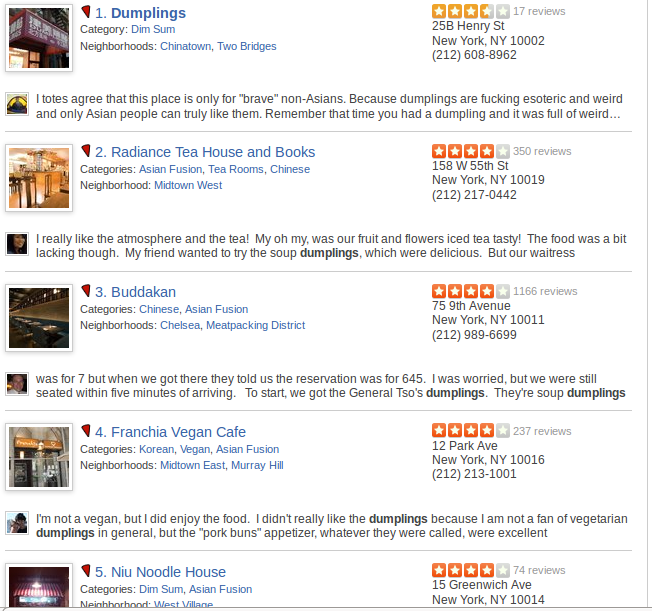
\includegraphics[width=0.5\textwidth]{fig/yelp.png}
  \caption{Yelp search results for "dumplings".
  Most of the top results have 4 stars, forcing users to read lengthy
  review text in order to gain better insight into quality.}
  \label{fig:yelp}
\end{figure}

Given a repository of social media data on a set of physical establishments,
the problem we address in this paper is how to best order establishments in 
a \emph{comparable category}.
Comparable categories are defined by a price point, type of restaurant, and coarse location.
For example, the Doughnut Plant in the Lower East Side would be categorized as <\$, donut\_shop, NYC>.
Per Se in Columbus Circle would be categorized as <\$\$\$\$, french\_restaurant, NYC>.
The type and price annotations are taken directly from Google Maps.

We cast our problem as a machine learning problem.
Social media attributes (e.g. review counts, ratings, check-in counts) are encoded as
features for each particular establishment.
A classifier or regressor model can then be trained to output quality scores for any
establishment. 
The model would output a discrete numerical value, which can be used to later
order places in a comparable category.
However the question remains, how should a training set be labeled
and what should be used as the absolute truth in quality judgement?

One approach is to directly use the average rating from all reviews of a place.
At first glance, using average review score may seem like an attractive
metric to directly use for ranking restaurants.
It is computationally inexpensive, easy to implement, compatible with
most search architectures, and provides significant information gain.
However, it comes with unacceptable long-term consequences:
\squishlist
\item {\bf Reinforcement of popular places} \\
Existing popular places are reinforced at the top of search results \cite{cho2004,cho2005}.
While this has been effectively used to improve Web search results \cite{xue2004},
its use in location-based search may make new high-quality places hard to discover.
This property leads to a substantial bias towards places that were first to become popular,
leading to sparse reviews for other places.
\item {\bf Low resolution of rating} \\
Rating systems tend to be very low resolution (i.e. a single rating from 0-5).
Websites struggle over the tradeoff between keeping the process simple and easy-to-use,
and gaining higher resolution into the different aspects of quality, such as food, service, and decor.
For this reason, a small Chinese dumpling shop in Chinatown has more reviews and the same number
of stars as one of the most critically-acclaimed restaurants in New York City.
It becomes unclear what does 4.5/5.0 stars mean.
A restaurant may have very high food quality, but offer a poorly decorated space.
A salon may offer fantastic service, but at an unreasonably high price.
\item {\bf Noisy data} \\
Users are notoriously inconsistent with their ratings \cite{chevalier2003effect}.
A single bad experience may lead a user to give an establishment 1 star, even when
the restaurant is on average reasonably good.
Additionally, each user has different personal interpretations of the meaning of each rated star,
leading to substantial noise in the final rating.
\squishend

Editorial rating services such as Zagat and Michelin address these limitations in a number of ways.
First, the decision to review a place is not directed by which places they have previously reviewed,
leading to a more even distribution of reviews among establishments.
Second, many provide greater insight into the components of quality with great resolution.
For example, Zagat produces an individual score from 0 to 30 separately for food, service, and decor.
Third, reviews are determined through a very strict and detailed methodology, many times with
the help of trained professionals.
Although not perfect, the result is more consistent ratings across a variety of establishments.

Editorial reviews are an incredibly sparse dataset.
The fact that editorial reviews require some element of human curation makes the service costly
and leads to the fact that only the top tier of establishments in the city get reviewed.
\emph{SolocoRank} labels training data with the aid of a particular editorial
review service (e.g. Zagat, Michelin).
Once trained, the model then is used to predict the editorial score of all restaurants in the United States
that haven't been officially rated by the editorial organization.

It would be easy to expect that a predicted editorial review score's ranking
would perform poorly, especially for long-tailed lower quality restaurants.
Individual features can be quite sparse.
For example, only 12\% of establishments in New York City have reviews.
The training data is also typically biased towards high quality or well-known
restaurants. 
However as shown in Section \ref{sec:evaluation},
we were surprised to find that predicted Zagat scores were able to
extrapolate well to all restaurants and
provide significant performance gains compared to just using average user ratings, even for the long-tail.
\emph{SolocoRank} leverages Google's large data repository to generate accurate models,
demonstrating that editorial reviews are a better general indicator
of consumer opinion.

\section{Quality Classification Using \\Social Media}
\label{sec:design}
\subsection{Overview}

\emph{SolocoRank} leverages a variety of data sources
to predict the editorial score of an establishment.
This score can then be used to rank establishments in a recommendation engine
or search engine.
Our goal is to create a query-independent score to improve performance
across a variety of different restaurant categories.
Our goal is not to produce any application-specific results or model
an individual's preferences to improve their search results.

Our hypothesis is that editorial reviews can be used to more accurately
order the quality of restaurant recommendations.
We calculate a \emph{SolocoRank} for each restaurant and bar in the United States,
which can be used as an additional signal for applications such as
recommendation engines and search engines.

That is not to say that \emph{SolocoRank} is an accurate representation of
the absolute real-world quality of an establishment.
In other words, the score generated is not meant to be displayed to the user.
\emph{SolocoRank} is also not meant to be used for a global ordering of all
restaurants. 
Instead, we evaluate the ability for \emph{SolocoRank} to accurately relatively
order restaurants within comparable categories of restaurants,
As mentioned in Section \ref{sec:setup}, comparable categories represent
restaurants with similar types of food in similar price ranges.

Our algorithm works as follows. 
We collect a list of all restaurants and bars in the United States that have
editorial scores.
We then aggregate a number of data sources (e.g. Google Maps, Google Plus,
Google Latitude, Web index).
In this aggregation phase, we count review statistics, and check-in statistics
for all restaurants.
We also use an entity annotator on all microblog posts (e.g. Google Plus, Twitter), and then
count statistics on how often restaurants are mentioned.
These results are then joined as features to the list of editorial-reviewed places.
We then train a classifier, using the discrete editorial score as labels.
Although regression could also be used, we were able to achieve better performance
using classifiers, as we demonstrate in Section \ref{sec:evaluation}.

We could have also bucketed editorial scores into fewer labels to improve
classifier accuracy, we found that less score-resolution actually hurt our
ability to order.
Thus, we attempt to just predict the exact editorial score of a restaurant
and use this score to order even restaurants that were never reviewed by 
the editorial organization.

There exist a number of key technical challenges to \emph{SolocoRank}.
Firstly, the features that we rely on are rather sparse.
While there were places with a very large number of reviews, 
most of the places we encountered had only a handful of reviews.
Features also had a strong location dependence.
In a high-tech hub of food culture like New York City,
far more places had user check-ins,
when compared to rural towns.
Furthermore, our training data of editorial-reviewed places
tended to be the types of places that had very strong signals, such as high review count.
Generalizing our model to work on any restaurant in the US proved to be a difficult task.
While we wanted to avoid overfitting, at the same time, our model needed to include
a vast amount of complex relationships.

Our proposed solution uses supervised learning.
We used the MapReduce \cite{mapreduce} framework to aggregate our large data sources
and train models in parallel. 
Due to the size of the data in question, it was important that our process was
fully automatic. 
Human relevance judgements were only used for generating our evaluation test sets.

\subsection{Features}
\label{sec:features}
We gather the following four types of features for each establishment
in the United States:
\squishlist
	\item \textbf{User reviews}\\
  We collect review counts and scores for all places registered in Google Maps.
  These include reviews from Google Maps core and Zagat.com user reviews.
  Just for the purposes of this paper evaluation, we also crawl a limited number of Yelp pages for their reviews.
  We also decompose these counts into additional features.
  For example, we count the number of users that gave the restaurant each particular rating.
	\item \textbf{Mentions}\\
  We use an entity annotator to detect restaurant names in arbitrary webpages.
  Using this, we can count the number of times the restaurant has been mentioned on the Web,
  as well as how many times it has been mentioned in Google Plus posts.
  Just for the purposes of this paper evaluation, we also crawl a limited number of popular Twitter pages.
	\item \textbf{Check-ins}\\
  We gather check-in data from Google Latitude.
  Just for the purposes of this paper evaluation, we also crawl a limited number
  of popular Foursquare pages for check-in counts.
  \item \textbf{Google Maps}\\
  As mentioned earlier, many of the aforementioned signals are location dependent.
  We encode the location as a feature, as well as any additional attributes that are
  stored in the Google Maps repository.
  This includes for example, the Pagerank of the associated webpage.
  It also contains a count of the number of photos and videos associated with a place.
\squishend

\subsection{Classifiers}
Because SolocoRank is a general machine learning-based framework,
we have the option of choosing from a variety of different classifiers.
Depending on what data sources are used and how features are encoded,
different classifiers may hold specific advantages.
Similarly, parameter-tuning may vary depending on the data.

In our implementation, we offer linear classifiers (e.g. Perceptron, Winnow),
decision trees (e.g. CART), ensemble classifiers (e.g. AdaBoost, TreeBoost, Random Forests),
and logistic regression.
In Section \ref{sec:classifierperformance}, we evaluate the accuracy and error
of each model for our data set.

\section{Evaluation}
\label{sec:evaluation}
We evaluated our ranking techniques using a large dataset
from real web services in deployment with data from real users.
We trained models on all Zagat-rated establishments in the US,
using the Zagat editorial score as ground truth label.
We performed three sets of experiments:
\squishlist
  \item Evaluation of accuracy and mean squared error of various classifiers
  \item Evaluation of performance of average user review rating
  \item Comparison of performance of SolocoRank-generated scores and various other metrics
\squishend
We also report on the dataset used and the experimental setup.

\subsection{Classifier Performance}
\label{sec:classifierperformance}
We evaluated a variety of classifiers and measured their accuracy and mean squared error.
Out of all of the Zagat-rated restaurants in the United States,
we randomly split half into a training set and half into a testing set.
Each classifier was trained on the training set, and then evaluated on the test set.
Mean squared error is only plotted for testing error.

\begin{figure}
  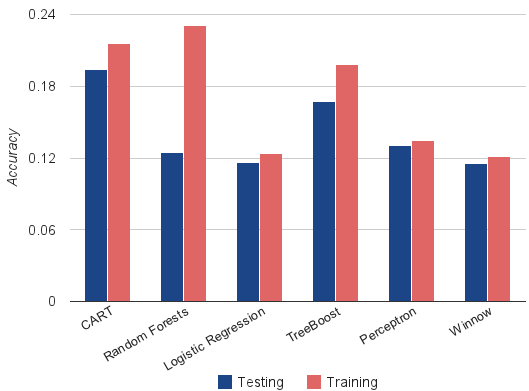
\includegraphics[width=.5\textwidth]{fig/classifieraccuracy.png}
  \caption{Classifier accuracy for various classifiers. 
  CART decision trees have the highest classification accuracy,
  predicting the exact Zagat score 19\% of the time.}
  \label{fig:classifieraccuracy}
\end{figure}

Figure \ref{fig:classifieraccuracy} shows the classifer accuracy.
Note that Zagat scores are discrete values from 0 to 30.
Thus, this chart represents each classifier's ability to
predict the Zagat score exactly.
Classification and regression trees (CART) are able to accurately 
predict the exact Zagat score about 19\% of the time.
CART was able to predict the Zagat score within $\pm1$ point, 44\% of the time.

\begin{figure}
  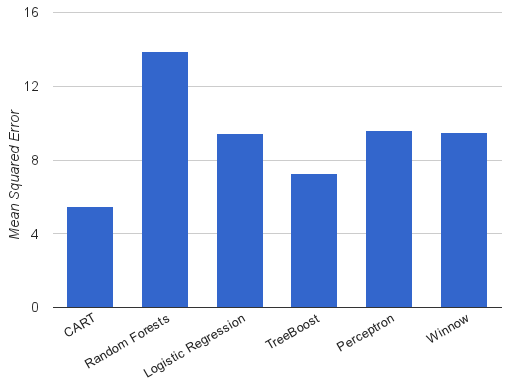
\includegraphics[width=.5\textwidth]{fig/meansqerror.png}
  \caption{Mean squared error of various classifiers on test set.
  CART decision trees have the lowest mean squared error of 5.46.}
  \label{fig:classifiermeansqerror}
\end{figure}

Figure \ref{fig:classifiermeansqerror} shows the mean squared error from each classifier.
CART again does the best along this metric.
With a mean square error of 5.46, this means that CART predictions are on average only a
few points off of the true Zagat score.

In general, decision tree-based classifiers performed better than others.
Trees are able to capture complex relationships, as well as produce a human-readable
tree that describes such relationships.
For example, a tree can capture the trend that checkin-based services 
are much more commonly used in certain cities than other places.
However in order to train our CART model, it took on the order of days to weeks depending
on the parameters.
The rest of the paper will evaluate \emph{SolocoRank} using the TreeBoost model with limited
complexity, allowing us to perform more evaluations with shorter training time.
As shown in Figures \ref{fig:classifieraccuracy} and \ref{fig:classifiermeansqerror},
TreeBoost performs close to the performance of CART.
In all experiments, we limited TreeBoost to 50 rounds of boosting,
where each tree was limited to a depth of 6.

\subsection{Generating Test Sets of Restaurants}
\subsubsection{Data Collection}
Our evaluation data consists of 150 test sets of five restaurants each.
In order to generate these sets, we divided all restaurants in New York City into comparable categories.

Once we had comprehensive restaurant coverage in each comparable category,
each comparable category was further divided into sets of five, labeled by the original category.
If a comparable category contains less than five elements, that category was disgarded.
We then selected 150 sets at random from all sets to compose the evaluation data set.
Thus, our evaluation data set distribution is approximately close to the distribution of restaurants
in existence in the city of New York.
However, note that this distribution of restaurants is likely different 
from the distribution of search queries on a mapping site.

This process was performed in order to produce query-independent sets of 
restaurants in the same comparable category.
Each set contains five random restaurants without any bias from an existing search engine.

\begin{figure}
  \begin{center}
    \begin{tabular}{|c|c|}
      \hline
      Restaurant Name           & Rating \\
      \hline
      \hline
      Shanghai Gourmet          & 3 \\
      \hline
      Xi'an Famous Foods        & 4 \\
      \hline
      Fong Inn Too              & 3 \\
      \hline
      Shu Jiao Fu Zhou Cuisine  & 3 \\
      \hline
      Oriental Kitchen          & 1 \\
      \hline
    \end{tabular}
  \end{center}
  \caption{Example of a test set in a comparable category: 
  cheap Chinese restaurants in New York City}
  \label{fig:testset}
\end{figure}

\subsubsection{Obtaining Relevance Ratings}
Each of these sets were then scored by three unique raters.
The rater was asked to assign a "relevance score" on a scale from [1-5] 
to each of the restaurants in a test set according to the following guidelines:
\squishlist
	\item 5 - You would frequently go or recommend this place to others
	\item 4 - You would definitely try this place at least once
	\item 3 - You may go to this place if it is in your area
	\item 2 - You would go to this place only in dire circumstances
	\item 1 - You would never go to this place
  
\squishend
Raters were encouraged to research these restaurants using a variety of online resources, 
including restaurant recommendations, Web search, newspaper articles, and user reviews.
The score may include a number of considerations, 
including the quality of food, cleanliness, service, and popularity. 
In the case where the restaurant type was misclassified 
(i.e. a French restaurant in a set of Chinese restaurants), 
the rater could still score the rest of the set, while ommiting the score of the misclassified restaurant.

Note that the rater was not asked to strictly order the restaurants. 
The set of five restaurants provides a frame of reference, but scores did not have to be unique.
Thus it was common to see repeat scores within a single set.
For example, a list of five restaurants may yield the scores [3, 4, 3, 3, 1]
as shown in Figure \ref{fig:testset}.

After each test set was scored by three raters, we ultimately took the majority 
as the final relevance score.
For example, if the raters returned: [3,4,3,3,1], [3,4,3,2,2], and [2,4,3,4,1], 
the final score was [3,4,3,x,1].
The fourth restaurant was disgarded from the set, 
because the raters could not come to a majority agreement.
We found that disagreement was generally very rare.

\subsubsection{Calculating Ranking Quality}
We evaluate a particular ranking method, such as \emph{SolocoRank}, by using the standard NDCG metric.
Given the relevance list of restaurants $R$ of a predicted ranking, 
the Discounted Cumulative Gain (DCG)
at position $p$ is given by $DCG_p(R) = \sum_{i=1}^{p}(2^{R_i}-1)/log_2(i+1)$.
This particular formulation of the DCG takes into account the rankings of the $p$ positions
and gives results at the top of the list more weight.
The normalized DCG (NDCG) can then be defined as $NDCG_p(R) = DCG_p(R)/DCG_p(I)$, where $I$ is
the relevance labeling of the ideal ranking.
Because each test set contains 5 restaurants, we always calculate NDCG for $p=5$.

\subsection{Raw User Review Scores}
In this section, we characterize raw user-generated reviews and 
evaluate the ability for user reviews to properly order restaurants.
User reviews are normalized on a scale from [0-100] and we simply take the average
review score across all reviews.
This average rating was then used to order our evaluation test sets,
without the use of machine learning.

\begin{figure}
  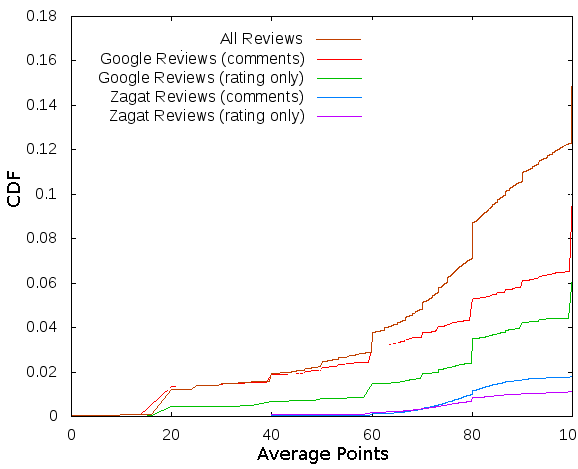
\includegraphics[width=0.5\textwidth]{fig/graph-avgpoints2.png}
  \caption{Cumulative distribution function (CDF) of average review scores in our database.
  CDF is shown separately for reviews with comments and reviews with only a star rating.
  CDF is also shown separately for Google Maps reviews and reviews from Zagat.com.
  Reviews are a sparse data set and users tend to have high score biases.}
  \label{fig:reviewscoredistribution}
\end{figure}

Figure \ref{fig:reviewscoredistribution} shows the cumulative 
distribution function of average review scores of establishments in the US.
The graph clearly shows that users tend to have strong biases towards high scores.
This property lowers the amount of information gained from users, while inflating scores shown to users.
Second, reviews are a scarce data source.
Roughly 12\% of establishments in New York City have any review scores associated with it.
Note that this is a percentage of all registered establishments in the city,
and not just bars and restaurants.

We then calculated the NDCG of our evaluation set,
using average user review score as the ranking metric.
Section \ref{sec:evaluation} describes our experimentation setup in greater detail.
As expected, ordering by average user review score provides
higher quality ordering of restaurants when compared to random ordering,
as shown in Figure \ref{fig:ndcgtable}.
The experiment yielded an average NDCG value of 0.8831,
across our evaluation data set, described in Section \ref{sec:setup}.

There were a few limitations to the approach.
In our experiments, an establishment with no score is treated 
the same as an establishment with a score of 0.
However, this may not reflect reality, as it inherently 
discriminates against new restaurants.
In the case where we had no reviews, there was no way to leverage other
forms of data to relatively order the restaurant.

Furthermore, the signal proved to be unreliable in the case where
there were only a few reviews. 
Suppose we were trying to relatively order two places, 
each with only a handful of reviews.
The average user review score is then a very noisy signal,
and it is very unlikely that both places were reviewed by the same people.

One could incorporate review counts in a more complex heuristic
for ranking.
However, this approach raises additional problems.
One could encounter a self-referring loop, where restaurants with many reviews
are reinforced at the top of search results and become hard to dislodge.
It also introduces the question of what heuristic should be used to 
combine this information in a way that reflects what users want.
\emph{SolocoRank} aims to solve exactly this problem by applying machine learning
to the problem.
In the next Section, we introduce the methodology behind \emph{SolocoRank},
which addresses these limitations and leads to further improvements in NDCG.

\subsection{NDCG Summary}
\begin{figure}
  \begin{center}
  \begin{tabular}{|c|c|}
    \hline
    Ranker            & NDCG  \\ \hline \hline
    Random            & 0.8393\\ \hline
    User Reviews      & 0.8831\\ \hline
    PlaceRank         & 0.8947\\ \hline
    \emph{SolocoRank}        & 0.8891\\ \hline
    \emph{SolocoRank}*PlaceRank  & 0.9011\\ \hline
  \end{tabular}
  \end{center}
  \caption{Average NDCG values across all test sets in our evaluation data.
  Due to high relevance score bias from our raters, NDCG values are biased high.
  However, both \emph{SolocoRank} and Google's current PlaceRank algorithms outperform
  using user-review scores. A linear combination of \emph{SolocoRank} and PlaceRank
  produces the highest quality scores.}
  \label{fig:ndcgtable}
\end{figure}

Figure \ref{fig:ndcgtable} summarizes average NDCG scores across our evaluation test sets.
Random ordering produces a rather high NDCG value of 0.839, 
due to the high score bias from our raters. 
Many times raters would return sets where a number of restaurants have either
high scores or identical scores. 
Due to the way NDCG is calculated, restaurants with the same relevance
can be ordered arbitrarily and still be perfectly ordered.
Because of this bias, the raw NDCG value provides little insight into
performance gains of \emph{SolocoRank}. In later sections, we use
non-parametric evaluations to highlight performance gains.
Even with such a high NDCG bias, we see that both \emph{SolocoRank} and
Google's current algorithm, PlaceRank, outperform user reviews.
As a point of comparison when we perform a linear combination of \emph{SolocoRank} and PlaceRank,
we show consistently better performance compared to any other individual signal.

\subsection{SolocoRank Quality}
In this section, we use the TreeBoost classifier to evaluate the NDCG
of \emph{SolocoRank} on the evaluation data.
We compare the performance of \emph{SolocoRank} to random ordering, average user review score,
and PlaceRank, Google's current state of the art algorithm.
Although our evaluation set contains only restaurants and bars in New York City,
our \emph{SolocoRank} model is trained on all Zagat-rated places in the United States.

\begin{figure}[h]
  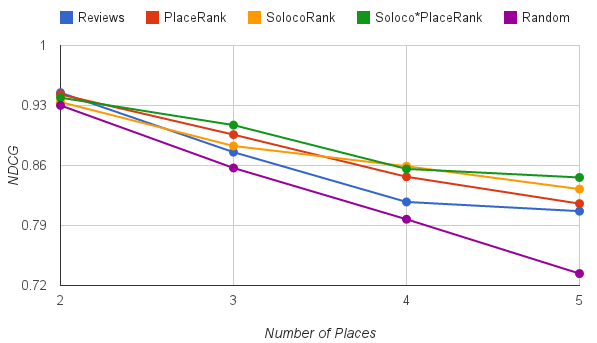
\includegraphics[width=.5\textwidth]{fig/ndcg-vs-numdocs.png}
  \caption{NDCG across varying numbers of documents. 
  \emph{SolocoRank} consistently outperforms using average user review scores.
  Due to the distribution of relevance scores, NDCG values had a high bias.}
  \label{fig:ndcg-vs-numdocs}
\end{figure}

Figure \ref{fig:ndcg-vs-numdocs} graphs the NDCG of the various methods
across different numbers of documents.
In other words, we vary $p \in [2,5]$, where $DCG_p(R) = \sum_{i=1}^{p}(2^{R_i}-1)/log_2(i+1)$.
Note that if all of the documents in the first $p$ elements of $R$
contain the same relevance score from the raters,
then the NDCG will always be 1, regardless of the ranker used.

Thus for lower values of $p$, NDCG values tended to be much higher and closer.
For larger values of $p$, we notice that \emph{SolocoRank} consistently performs better
than user reviews.

\begin{figure}[h]
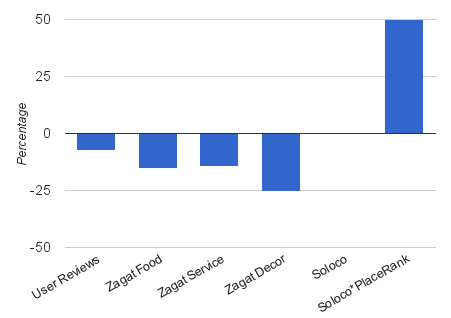
\includegraphics[width=.5\textwidth]{fig/versusplacerank.png}
\caption{When counting the number of test sets for which SolocoRank
had a higher NDCG, we show that each individual review signal performed
worse than SolocoRank by 10-25\%}
\label{fig:versusplacerank}
\end{figure}

Due to the distribution of relevance scores that were assigned in our
evaluation test set, NDCG values had a substantial high bias, even for random ordering.
Thus, it was helpful to perform non-parametric evaluations of each method.
In these evaluations, we counted the number of test sets, where the NDCG is higher
for \emph{SolocoRank}, when compared to the NDCG from average user reviews.
Figure \ref{fig:versusplacerank} shows the percentage improvement in the 
number of test sets with a higher NDCG value when compared to SolocoRank.
For example when SolocoRank was compared to PlaceRank, there were equal
numbers of test sets where the NDCG value was higher for SolocoRank, as
there were test sets where the NDCG value was higher for PlaceRank.
However, it is interesting to note that any individual review signal performed
worse than SolocoRank.
When using user review scores, there was about 10\% fewer test sets with better
NDCG.
Again as a point of comparison, we were able to show 50\% improvement
when SolocoRank was combined with PlaceRank.

\subsection{Information Gain from Social Media}
\begin{figure}[h]
  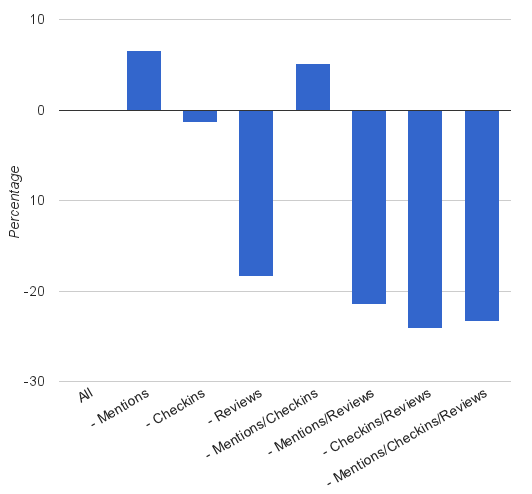
\includegraphics[width=.5\textwidth]{fig/signalselection-accuracy.png}
  \caption{Classifier accuracy without particular features. As expected,
  reviews provide the most information gain. Surprisingly, classifier
  accuracy performs better without \emph{mention} data.}
  \label{fig:signalselection-accuracy}
\end{figure}

We wanted to evaluate the effect of each particular category of signals in 
the final NDCG value.
Figure \ref{fig:signalselection-accuracy} shows the percent change in NDCG, 
compared to the original baseline of using all signals.
As expected, removing reviews severely impaired SolocoRank's NDCG performance.
However, it was surprising to see that the removal of mentions actually improved
NDCG performance.
This negative effect may be caused by the way this signal was produced and encoded.
At the moment, we simply count the number of mentions on Google Plus
and Twitter webpages with a minimum PageRank value.
In the future, we could perform more intelligent sentiment analysis in conjunction with
mentions in order to determine if the mention was negative or positive.

\section{Discussion}
\label{sec:discussion}
In this Section, we discuss different varieties of how
\emph{SolocoRank} can be computed, which may lead to substantially different results.

\subsection{Localized Classifiers}

\begin{figure}[h]
  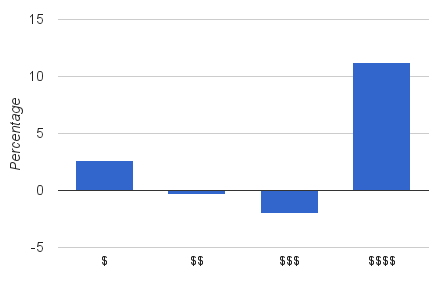
\includegraphics[width=.5\textwidth]{fig/ndcg-vs-price.png}
  \caption{Percentage improvement of \emph{SolocoRank} NDCG values in a particular
  price bracket in comparison to the overall NDCG value. NDCG values are
  higher for the highest-tier and lowest-tier of prices.}
  \label{fig:ndcg-vs-price}
\end{figure}

As is the case with most machine learning applications,
\emph{SolocoRank} is highly dependent on how features are represented
and various parameters that dictate how the model is composed.
For example, we noticed early on that \emph{SolocoRank} performs
substantially better for high-priced restaurants.
Figure \ref{fig:ndcg-vs-price} shows the average NDCG values,
when test sets are separated by price point.

We can attribute this to two factors. 
First of all, our training data highly depends on which restaurants
that Zagat chooses to rate.
At the moment, this decision is something we do not have any insight into.
Second, the consumer behavior is highly complex, dynamic, and in many times hard to capture.
The act of checking in is a very new phenomenon and may not be as
prevalent in certain cities or in certain classes of society.

\begin{figure}[h]
  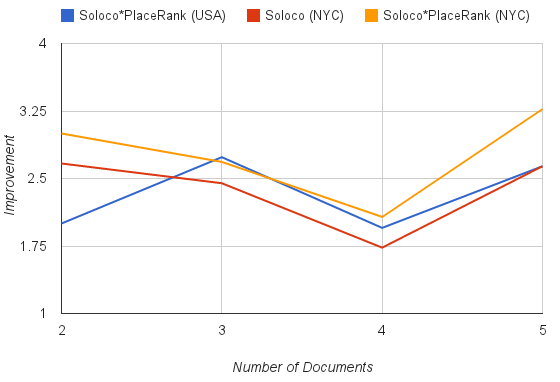
\includegraphics[width=.5\textwidth]{fig/localclassifier.png}
  \caption{Performance gains when training on only local data (New York City). 
  We count the number of test sets where the NDCG is higher for SolocoRank, compared
  to user review scores.
  Local classifiers perform 2-3 times better than a general model trained on all
  US Zagat data.}
  \label{fig:localclassifier}
\end{figure}

In the case of location, we wanted to evaluate the performance of \emph{SolocoRank},
trained only on local data. In other words, we removed location as a feature
and trained a classifier only on Zagat-rated restaurants in the New York City area.
Figure \ref{fig:localclassifier} shows the result of this evaluation.
We plot the improvement in the number of test sets where the NDCG was higher over \emph{SolocoRank}.
When \emph{SolocoRank} was only trained on local NYC places, 
there was a 2-3 times improvement over a general model trained on
all data in the US.

While it would be nice to have one general classifier,
it may be advantageous to train separate localized classifiers for each 
major metropolitan area due to the complex nature of location.
Further evaluation would need to be performed to argue whether
this is true of any other feature, such as price bracket.
However, this decision must be made with care, as the space of
classifiers quickly explode with more localization.

\subsection{Additional Data Sources}
In all of our evaluations, we only use features based on counts and
discrete assigned scores.
However, research has shown that free-form text may contain
valuable information that acts as strong signals for recommendations \cite{ganu2009}.
Future work ought to use advanced sentiment analysis techniques on reviews
to generate more features and strengthen the model.

Furthermore, as users are increasingly relying on online mapping services,
we can use a variety of new signals from these services.
For example, we use click-through data or even count the number of times
a user gets directions to a particular establishment.

\subsection{Alternative Labels}
In this paper, we make the assumption that Zagat is ultimately the ground truth
in quality distinctions.
This allows us to evaluate our ranker on relevance scores from external raters.
However, Zagat scores could instead be encoded as features.

Because \emph{SolocoRank} is a general learn-to-rank architecture,
any other score could be used as the training labels.
This could include other editorial review services, or even the rater's
relevance scores directly.
It is an open question, which signal most accurately reflects 
general consumer opinion on quality.


\section{Conclusions}
\label{sec:conclusion}

In this paper, we presented a solution for 
producing quality scores for physical establishments such as 
restaurants and bars.
This score can be used to order places, improving the performance
of applications such as recommendation engines and local search.
By using machine learning techniques to train a model on trusted
editorial reviews and social media data,
the model can accurately predict the expected editorial score
in the absense of an official score.
\emph{SolocoRank} inherently leverages a variety of different data sources
and does not rely on any one particular form of user-generated data.
\emph{SolocoRank} can easily be later adapted to other forms of data,
as users evolve the way they provide feedback on restaurants.
Many opportunities exist to improve on our existing work,
such as producing localized classifiers for each city,
or using other forms of feature encoding and data sources.
Overall, our techniques help unveil important information
that gives web services a unique ability to judge establishments
for improved user recommendations on websites.

\newpage
%%ACKNOWLEDGMENTS are optional
\section{Acknowledgments}
We are grateful to TODO [INSERT NAMES]
for helpful discussions and valuable feedback

%\end{document}  % This is where a 'short' article might terminate

%
% The following two commands are all you need in the
% initial runs of your .tex file to
% produce the bibliography for the citations in your paper.

%\bibliographystyle{abbrv}
%\bibliography{paper}  % sigproc.bib is the name of the Bibliography in this case
{\small \bibliographystyle{abbrv}
\bibliography{paper}}  % sigproc.bib is the name of the Bibliography in this case

% You must have a proper ".bib" file
%  and remember to run:
% latex bibtex latex latex
% to resolve all references
%%APPENDICES are optional
%\balancecolumns
\appendix
%Appendix A
\section{Headings in Appendices}
The rules about hierarchical headings discussed above for
the body of the article are different in the appendices.
In the \textbf{appendix} environment, the command
\textbf{section} is used to
indicate the start of each Appendix, with alphabetic order
designation (i.e. the first is A, the second B, etc.) and
a title (if you include one).  So, if you need
hierarchical structure
\textit{within} an Appendix, start with \textbf{subsection} as the
highest level. Here is an outline of the body of this
document in Appendix-appropriate form:
\subsection{Introduction}
\subsection{The Body of the Paper}
\subsubsection{Type Changes and  Special Characters}
\subsubsection{Math Equations}
\paragraph{Inline (In-text) Equations}
\paragraph{Display Equations}
\subsubsection{Citations}
\subsubsection{Tables}
\subsubsection{Figures}
\subsubsection{Theorem-like Constructs}
\subsubsection*{A Caveat for the \TeX\ Expert}
\subsection{Conclusions}
\subsection{Acknowledgments}
\subsection{Additional Authors}
This section is inserted by \LaTeX; you do not insert it.
You just add the names and information in the
\texttt{{\char'134}additionalauthors} command at the start
of the document.
\subsection{References}
Generated by bibtex from your ~.bib file.  Run latex,
then bibtex, then latex twice (to resolve references)
to create the ~.bbl file.  Insert that ~.bbl file into
the .tex source file and comment out
the command \texttt{{\char'134}thebibliography}.
% This next section command marks the start of
% Appendix B, and does not continue the present hierarchy
\section{More Help for the Hardy}
The acm\_proc\_article-sp document class file itself is chock-full of succinct
and helpful comments.  If you consider yourself a moderately
experienced to expert user of \LaTeX, you may find reading
it useful but please remember not to change it.
\balancecolumns


%
% ACM needs 'a single self-contained file'!
%
% That's all folks!
\end{document}
